\documentclass[crop,tikz]{standalone}% 'crop' is the default for v1.0, before it was 'preview'
%\usetikzlibrary{...}% tikz package already loaded by 'tikz' option
\usepackage{color}
\newcommand{\gv}[1]{\ensuremath{\mbox{\boldmath$ #1 $}}} 
\renewcommand{\v}[1]{\ensuremath{\mathbf{#1}}}
\newcommand{\name}[1]{_{\text{#1}}}
\usepackage{siunitx}
\usetikzlibrary{shapes,arrows,shadings,backgrounds,calc}
\definecolor{brown}{rgb}{0.59, 0.29, 0.0}
\input{molecule_defs.tex}
\tikzstyle{decision} = [diamond, draw, fill=blue!20, 
    text width=6em, text badly centered, node distance=3cm, inner sep=0pt]
\tikzstyle{block} = [rectangle, draw, fill=blue!20, 
    text width=5em, text centered, rounded corners, minimum height=4em]
\tikzstyle{line} = [draw, -latex']
\tikzstyle{cloud} = [draw, ellipse,fill=red!20, node distance=3cm,
  minimum height=2em]

\begin{document}
\fontfamily{cmss}{\begin{tikzpicture}
        %Grid for drawing, comment out
  \node[anchor=south west](boundingbox)at(3.5,-11){\begin{tikzpicture}\draw[white,step=1cm,very thin] (0,6.) grid (15cm,-5cm);\end{tikzpicture}};
        %PART 1
  \node[scale=1.1](a)at (6,-2.45){\begin{tikzpicture}
      
        %Box with polymers
      %% \draw[ultra thick,gray] (0,0) rectangle (5cm,-5cm);        
      %%  \draw[ultra thick,rounded corners=10] (0,0)  rectangle (5cm,-5cm);

        %Polymers
        \node[scale=0.3,opacity=.5,rotate=30] (a6) at (2,-1) {\begin{tikzpicture}
  \node[wat4,scale=1.5] (wat1) at  (0,0) {};
  \node[wat4,scale=1.5] (wat2) at (0.5,-1) {};
  \node[wat4,scale=1.5] (wat3) at (0.0,-2) {};
  \node[carbon,scale=1.5] (carbon1) at (0.5,-3) {};
  \node[carbon,scale=1.5] (carbon2) at (0,-4) {};
  \node[carbon,scale=1.5] (carbon3) at (0.5,-5) {};
  \GreenBond{wat1}{wat2}
  \GreenBond{wat2}{wat3}
  \GreenBond{carbon1}{wat3}
  \GreenBond{carbon1}{carbon2}
  \GreenBond{carbon2}{carbon3}
\end{tikzpicture}
};
        \node[scale=0.3,opacity=.5,rotate=100] (a5) at (3.2,-2) {\begin{tikzpicture}
  \node[wat4,scale=1.5] (wat1) at  (0,0) {};
  \node[wat4,scale=1.5] (wat2) at (0.5,-1) {};
  \node[wat4,scale=1.5] (wat3) at (0.0,-2) {};
  \node[carbon,scale=1.5] (carbon1) at (0.5,-3) {};
  \node[carbon,scale=1.5] (carbon2) at (0,-4) {};
  \node[carbon,scale=1.5] (carbon3) at (0.5,-5) {};
  \GreenBond{wat1}{wat2}
  \GreenBond{wat2}{wat3}
  \GreenBond{carbon1}{wat3}
  \GreenBond{carbon1}{carbon2}
  \GreenBond{carbon2}{carbon3}
\end{tikzpicture}
};
        \node[scale=0.3,opacity=.5,rotate=66] (a0) at (1.1,-2.2) {\begin{tikzpicture}
  \node[wat4,scale=1.5] (wat1) at  (0,0) {};
  \node[wat4,scale=1.5] (wat2) at (0.5,-1) {};
  \node[wat4,scale=1.5] (wat3) at (0.0,-2) {};
  \node[carbon,scale=1.5] (carbon1) at (0.5,-3) {};
  \node[carbon,scale=1.5] (carbon2) at (0,-4) {};
  \node[carbon,scale=1.5] (carbon3) at (0.5,-5) {};
  \GreenBond{wat1}{wat2}
  \GreenBond{wat2}{wat3}
  \GreenBond{carbon1}{wat3}
  \GreenBond{carbon1}{carbon2}
  \GreenBond{carbon2}{carbon3}
\end{tikzpicture}
};
        \node[scale=0.3,opacity=.5,rotate=60] (a1) at (1,-3.5) {\begin{tikzpicture}
  \node[wat4,scale=1.5] (wat1) at  (0,0) {};
  \node[wat4,scale=1.5] (wat2) at (0.5,-1) {};
  \node[wat4,scale=1.5] (wat3) at (0.0,-2) {};
  \node[carbon,scale=1.5] (carbon1) at (0.5,-3) {};
  \node[carbon,scale=1.5] (carbon2) at (0,-4) {};
  \node[carbon,scale=1.5] (carbon3) at (0.5,-5) {};
  \GreenBond{wat1}{wat2}
  \GreenBond{wat2}{wat3}
  \GreenBond{carbon1}{wat3}
  \GreenBond{carbon1}{carbon2}
  \GreenBond{carbon2}{carbon3}
\end{tikzpicture}
};
        \node[scale=0.3,opacity=.5,rotate=-90] (a4) at (3.5,-0.5) {\begin{tikzpicture}
  \node[wat4,scale=1.5] (wat1) at  (0,0) {};
  \node[wat4,scale=1.5] (wat2) at (0.5,-1) {};
  \node[wat4,scale=1.5] (wat3) at (0.0,-2) {};
  \node[carbon,scale=1.5] (carbon1) at (0.5,-3) {};
  \node[carbon,scale=1.5] (carbon2) at (0,-4) {};
  \node[carbon,scale=1.5] (carbon3) at (0.5,-5) {};
  \GreenBond{wat1}{wat2}
  \GreenBond{wat2}{wat3}
  \GreenBond{carbon1}{wat3}
  \GreenBond{carbon1}{carbon2}
  \GreenBond{carbon2}{carbon3}
\end{tikzpicture}
};               
        \node[scale=0.3,opacity=.5,rotate=0] (a2) at (4.2,-3.5) {\begin{tikzpicture}
  \node[wat4,scale=1.5] (wat1) at  (0,0) {};
  \node[wat4,scale=1.5] (wat2) at (0.5,-1) {};
  \node[wat4,scale=1.5] (wat3) at (0.0,-2) {};
  \node[carbon,scale=1.5] (carbon1) at (0.5,-3) {};
  \node[carbon,scale=1.5] (carbon2) at (0,-4) {};
  \node[carbon,scale=1.5] (carbon3) at (0.5,-5) {};
  \GreenBond{wat1}{wat2}
  \GreenBond{wat2}{wat3}
  \GreenBond{carbon1}{wat3}
  \GreenBond{carbon1}{carbon2}
  \GreenBond{carbon2}{carbon3}
\end{tikzpicture}
};
        \node[scale=0.3,opacity=1,rotate=90] (main) at (3,-3) {\begin{tikzpicture}
  \node[wat4,scale=1.5] (wat1) at  (0,0) {};
  \node[wat4,scale=1.5] (wat2) at (0.5,-1) {};
  \node[wat4,scale=1.5] (wat3) at (0.0,-2) {};
  \node[carbon,scale=1.5] (carbon1) at (0.5,-3) {};
  \node[carbon,scale=1.5] (carbon2) at (0,-4) {};
  \node[carbon,scale=1.5] (carbon3) at (0.5,-5) {};
  \GreenBond{wat1}{wat2}
  \GreenBond{wat2}{wat3}
  \GreenBond{carbon1}{wat3}
  \GreenBond{carbon1}{carbon2}
  \GreenBond{carbon2}{carbon3}
\end{tikzpicture}
};     

        %BLUE square
        \draw[ultra thick,dashed,opacity=1,blue,rounded corners=20] ([xshift=-2cm,yshift=-1cm]main.south west) rectangle ([xshift=2cm,yshift=0.75cm]main.north east); 

        %Visible polymer
        \node[scale=0.3,opacity=1,rotate=90,blue] (main) at (3,-3) {\begin{tikzpicture}
  \node[wat4,scale=1.5] (wat1) at  (0,0) {};
  \node[wat4,scale=1.5] (wat2) at (0.5,-1) {};
  \node[wat4,scale=1.5] (wat3) at (0.0,-2) {};
  \node[carbon,scale=1.5] (carbon1) at (0.5,-3) {};
  \node[carbon,scale=1.5] (carbon2) at (0,-4) {};
  \node[carbon,scale=1.5] (carbon3) at (0.5,-5) {};
  \GreenBond{wat1}{wat2}
  \GreenBond{wat2}{wat3}
  \GreenBond{carbon1}{wat3}
  \GreenBond{carbon1}{carbon2}
  \GreenBond{carbon2}{carbon3}
\end{tikzpicture}
};     
        \node[blue] at ([xshift=-0.5cm,yshift=0.4cm]main) {\large $H_{0}$};
        \node[blue] at ([xshift=-0.1cm,yshift=-0.6cm]main) {\large $\{\v r,\dot{\v r}\}_m$};
        
        %Interactions
        \draw[<->,ultra thick,brown] (main)--(a2);
        \draw[<->,ultra thick,brown] (main)--(a1);
        \draw[<->,ultra thick,brown] (main)--(a5);
        \node[brown] at(0.75,-4.75){\large $W[\phi]$};
          \end{tikzpicture}
    
  };
  \node[anchor=north west]  at([xshift=0.2cm,yshift=-0.4cm] a.north west){\Large A}; 
       
  \draw[black,rounded corners=10,ultra thick] (a.south east)rectangle(boundingbox.north west);
        
        %Part 2
        
        \node(e) at (17,-5){
          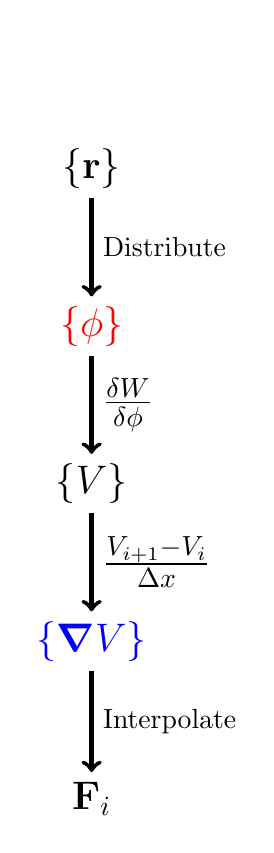
\begin{tikzpicture}
            \node[white]at (-0,1.5){\Large C};
            \node(a) at (0,0) {\Large $\{\v r\}$};
            \node[red](b) at (0,-2) {\Large $\{\phi\}$};
            \node[](c) at (0,-4) {\Large \{$V\}$};         
            \node[blue](d) at (0,-6) {\Large $\{\gv\nabla V\}$};
            \node[](e) at (0,-8) {\Large $\v F_i$};
           
            \draw[->,ultra thick] (a) --node[right]{Distribute}(b);
            \draw[->,ultra thick] (b) -- node[right]{\Large$\frac{\delta W}{\delta\phi}$}(c);
            \draw[->,ultra thick] (c) --node[right]{\Large$\frac{V_{i+1}-V_i}{\Delta x}$}(d);
            \draw[->,ultra thick] (d) --node[right]{Interpolate}(e);
          \end{tikzpicture}
          };

          \node[anchor=north west]  at([xshift=0.2cm,yshift=-0.4cm] e.north west){\Large C}; 

        \draw[black,rounded corners=10,ultra thick] (e.north west)rectangle(boundingbox.south east);


        %Single bead
        \node(g) at (12,-2.5){\begin{tikzpicture}
            \node at(4.75,-0.25){\Large B};
          \node[wat4,minimum size=7mm, ] (wat) at (7cm,-3.cm){};

        %Filled area
        \draw[fill=gray,opacity=0.4,draw opacity=0] (wat) rectangle (6cm,-1cm);
        \draw[fill=gray,opacity=0.9,draw opacity=0] (wat) rectangle (6cm,-4cm);
        \draw[fill=gray,opacity=0.4,draw opacity=0] (wat) rectangle (9cm,-4cm);
        \draw[fill=gray,opacity=0.1,draw opacity=0] (wat) rectangle (9cm,-1cm);
        \draw[ultra thick,dashed] (wat) -- (7,-1);
        \draw[ultra thick,dashed] (wat) -- (7,-4);        
        \draw[ultra thick,dashed] (wat) -- (9,-3);
        \draw[ultra thick,dashed] (wat) -- (6,-3);        

        
        %Grid
        \draw[ultra thick] (6cm,0cm) -- (6cm,-5cm);
        \draw[ultra thick] (9cm,0cm) -- (9cm,-5cm);
        \draw[ultra thick] (5cm,-4cm) -- (10cm,-4cm);
        \draw[ultra thick] (5cm,-1cm) -- (10cm,-1cm);

        
        %Single bead again
        \node[wat4,minimum size=7mm] (wat) at (7cm,-3.cm){};

        %Densities
        \node[red] at(5.5,-4.5){\Large$\phi_{11}$};
        \node[red] at(9.5,-4.5){\Large$\phi_{12}$};
        \node[red] at(5.5,-0.5){\Large$\phi_{21}$};
        \node[red] at(9.5,-0.5){\Large$\phi_{22}$};

        \draw[fill=red,red] (6.,-4)circle (0.1cm); 
        \draw[fill=red,red] (9.,-4)circle (0.1cm);
        \draw[fill=red,red] (6.,-1)circle (0.1cm);
        \draw[fill=red,red] (9.,-1)circle (0.1cm);

        
        %External field
        \node[blue,label={above,blue}:{\Large$\gv\nabla V_{\frac322}$}] at(7.5,-1){\Large$\gv\times$};
        \node[blue,label={below,blue}:{\Large$\gv\nabla V_{\frac321}$}] at(7.5,-4){\Large$\gv\times$};
        \node[blue,label={left,blue,xshift=+0.3cm}:{\Large$\gv\nabla V_{1\frac32}$}] at(6,-2.5){\Large$\gv\times$};
        \node[blue,label={right,blue,xshift=-0.25cm}:{\Large$\gv\nabla V_{2\frac32}$}] at(9,-2.5){\Large$\gv\times$};
        \end{tikzpicture}};

        \draw[black,rounded corners=10,ultra thick] (g.south west)rectangle(g.north east);
        
        %Part 3 Parallelization
        \node(c) at (9.5,-8.2){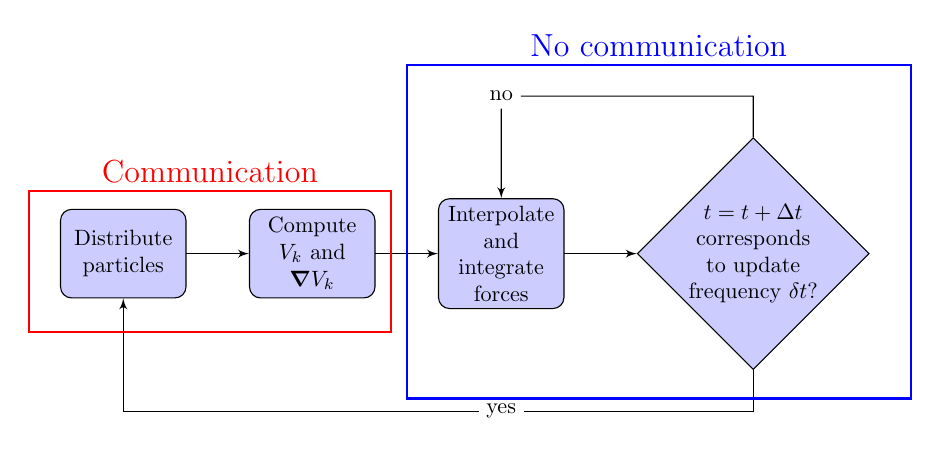
\begin{tikzpicture}[node distance = 2cm, auto,scale=0.8, every node/.style={scale=0.8}]
  % Place nodes
           % \node[]at (-1,3){\Large D};

  \node [block] (init) {Distribute particles};

  \node [block, right
    of=init,node distance=3cm] (solve) {Compute $V_k$ and $\gv \nabla
    V_k$};

  \node [block, right of=solve,node distance=3cm] (forces)
        {Interpolate and integrate forces};

  \node [decision, right of=forces,node distance=4cm] (new)
        {$t=t+\Delta t$ corresponds to update frequency $\delta t$?};


        \node [ below of=forces,node distance=2.5cm] (yes) {yes};
        \node [ above of=forces,node distance=2.5cm] (no) {no};

        \path [line] (new) |- (yes) -| (init);
        \path [line] (new) |- (no) -- (forces);
        %\path [line] (new) -- node [below forces] {no} (a);% -- ([xshift=-3.25cm])-- (solve);
       % \path [line, above] (new) -- (solve);
        \path [line] (init) -- (solve);
        \path [line] (solve) -- (forces);
        \path [line] (forces) -- (new);
        
        %% \path [line] (forces) |- (new);
    %% \path [line] (new) -| (init);


    \draw[blue,thick] (4.5,-2.3) rectangle (12.5,3);
    \draw[red,thick] (4.25,-1.25) rectangle (-1.5,1);
    \node[red,above](communication) at (1.375,1) {\Large Communication};
    \node[blue,above](communication2) at (8.5,3) {\Large No communication};
          \end{tikzpicture}
        };
        \node[anchor=north west]  at([xshift=0.2cm,yshift=-0.4cm]c.north west){\Large D};
        \draw[black,rounded corners=10,ultra thick] (boundingbox.south west)rectangle(c.north east);
        
\end{tikzpicture}}
\end{document}
